\documentclass[a4paper]{article} %\documentclass[]{article}
\usepackage[utf8]{inputenc}
\usepackage{graphicx}
\usepackage{float} % H positioning
\usepackage{lscape}

\usepackage{listings}

% head and footer
\usepackage{fancyhdr}
\pagestyle{fancy}
\fancyhf{}
\fancyhead[LE,RO]{\thepage}
\fancyhead[RE,LO]{\leftmark}
%\fancyfoot[CE,CO]{\leftmark}
%\fancyfoot[LE,RO]{\thepage}
\fancyfoot[LE,RO]{\thepage}
\fancyfoot[RE,LO]{\rightmark}
\renewcommand{\headrulewidth}{2pt}
\renewcommand{\footrulewidth}{1pt}


%code
\usepackage{lmodern}  % for bold teletype font
\usepackage{amsmath}  % for \hookrightarrow
\usepackage{amssymb} % for math symbols
\usepackage{xcolor}   % for \textcolor

\lstloadlanguages{Ruby}
\definecolor{ao(english)}{rgb}{0.0, 0.5, 0.0}
\lstset{
	basicstyle=\ttfamily,
	columns=fullflexible,
	frame=single,
	breaklines=true,
	postbreak=\mbox{\textcolor{red}{$\hookrightarrow$}\space},
	commentstyle = \ttfamily\color{gray},
	keywordstyle=\ttfamily\color{blue},
	stringstyle=\color{ao(english)},
	showstringspaces=false
}

\usepackage[hidelinks]{hyperref}


\begin{document}
	
	%opening
	\begin{titlepage}
		\centering
		\vspace*{1cm}
		%\includegraphics[width=0.20\textwidth]{images/logo_unipd.png}\par\vspace{1cm}
		{\par \scshape\LARGE Università degli Studi di Padova \par}
		\vspace{1cm}
		{\scshape\Large Dipartimento di Ingegneria dell'Informazione\\Corso di Laurea Magistrale in Ingegneria Informatica\par}
		\vspace{1.5cm}
		{\huge\bfseries Online contextual system tuning with Bayesian Optimization and Workload Forecasting\par}
		\vspace{2cm}
		{ \large \itshape Laureando:}
		{ \large Luca \textsc{Moroldo} \par}
		\vspace{0.7cm}
		{ \large \itshape Relatore:}
		{ \large Prof. Nicola \textsc{Ferro} \par}
		\vfill
		
		% Bottom of the page
		{ \large 25 Settembre 2019 \par}
		{ \large \textsc{Anno Accademico 2018/2019}\par}
	\end{titlepage}
	
	% empty page
	\clearpage%
	\thispagestyle{empty}%
	\addtocounter{page}{-1}%
	\null%
	\clearpage
	
	\newpage
	\pagenumbering{roman}
	\thispagestyle{plain}
	\section*{Sommario}
	
	L'oggetto della presente tesi è lo sviluppo del backend di un progetto realizzato durante una attività di tirocinio presso l'azienda Moku srl.\\
	Il progetto, consistente in una piattaforma web il cui utilizzo è destinato a scuole medie e superiori in Europa, sarà reso pubblico a inizio anno 2020 con l'intento di promuovere lo svolgimento di attività sportive all'interno degli ambienti scolastici; verranno discusse le fasi di modellazione ed implementazione del progetto in accordo con le specifiche fornite dal committente.\\\\
	Verranno presentate le metodologie e gli strumenti utilizzati per lo sviluppo con particolare attenzione verso GraphQL, un componente che ha ricoperto un ruolo di primaria importanza nello scambio di informazioni tra i client e il server grazie alle sue innovative caratteristiche ed ai vantaggi derivanti dal suo impiego. Verranno analizzate alcune debolezze prestazionali che affliggono l'implementazione delle specifiche di GraphQL per il linguaggio di programmazione Ruby e come queste debolezze siano state superate attraverso una estensione di tale implementazione.\\\\ 
	Verrà inoltre presentato uno strumento creato con lo scopo di automatizzare la produzione di codice relativo all'esposizione di dati ed operazioni da parte del backend sviluppato; questo strumento, che consente di evitare la scrittura di codice ridondante ma necessario, è stato incluso nelle risorse utilizzate dall'azienda assieme all'estensione dell'implementazione delle specifiche di GrahQl per il linguaggio Ruby.\\\\
	Il completamento del progetto è avvenuto nel rispetto delle tempistiche del tirocinio svolto.
	
	
	% empty page
	\clearpage%
	\thispagestyle{empty}%
	\addtocounter{page}{-1}%
	\null%
	\clearpage
	
	% Custom TOC title
	\renewcommand{\contentsname}{Indice}
	\newpage
	\thispagestyle{plain}
	\tableofcontents

	% empty page
	\clearpage%
	\thispagestyle{empty}%
	\addtocounter{page}{-1}%
	\null%
	\clearpage
	
	
	% =================== INTRODUZIONE ==========================
	
	\newpage
	\pagenumbering{arabic}
	
	\section{ Introduction }

	\section{ State of the art }
	
	\subsection{ System optimization }
	
	\subsection{ Forecasting }
	Forecasting is a common data science task that makes use of temporal data \cite{ForecastingSurvey} to help organizations with capacity planning, goals setting, and anomaly detection. It is required in many situations: for example, deciding whether to build another warehouse in the next five years requires forecasts of future demand, and scheduling staff in a call center next week requires forecasts of call volumes.
	
	The first successful forecasting methods have been proposed around \textit{1950}, some of them being Exponential Smoothing \cite{ExponentialSmoothingHoltCharles} and ARIMA \cite{ForecastingBoxJenkins}, which originated a wide variety of derived techniques \cite{25YearsForecasting}. In the big-data era, where companies have huge numbers of time series each with their own characteristics, traditional techniques have shown some limitations due to specific model requirements [\ref{sssec:exponential_smoothing}, \ref{sssec:arma}], model inflexibility, necessity of manual feature engineering, lack of automation, difficulties of dealing with missing data, and lack of well-performing multivariate models \cite{25YearsForecasting}.\\
	Recent developments have seen pure deep learning models joining the fields with inconsistent performance \cite{DeepLearningForecastingSurvey}, but highlighting the possibility of exploiting huge datasets in order to learn a single global model capable of recognizing complex and sometimes shared time series patterns. Other recent deep learning research achievements, especially in the natural language processing domain \cite{RNNLSTM, seq2seq, EncoderDecoder}, have inspired promising models \cite{DeepAR, DeepState, DeepLearningForecastingSurvey}, some of them having an hybrid architecture that utilizes both statistical and machine learning (ML) features \cite{MAKRIDAKIS2018802, GluonTS}. 
	Interestingly, the winner of the 2018 M4 competition \cite{MAKRIDAKIS2018802} was a combination of Exponential Smoothing and deep learning \cite{UberHybridES}, while the top-performing submissions of the 2020 M5 competition \cite{M5Competition}, where most of the time series have some kind of correlation and share frequency and domain, cross-learning ML models have shown their potential with the top-performing submissions using a weighted average of several pure ML models.\\
	Other methods, such as the one chosen by Prophet \cite{FacebookProphet}, provide an analyst-in-the-loop approach suggesting that by injecting domain-specific knowledge into the model it's still possible to outperform fully automated approaches, especially with small amounts of data .\\
	Nevertheless, Artificial Neural Network (ANN) based models have only recently started overtaking simpler classical models \cite{MAKRIDAKIS2018802, M5Competition} opening a set of inspiring possibilities, and the market has seen big companies developing their own solutions \cite{FacebookProphet, GluonTS, MicrosoftSSA, UberHybridES}, highlighting the necessity for the businesses of better forecasting techniques.
	
	Despite the forecasting importance, there are still serious challenges associated with producing reliable and high quality forecasts: time series often have long term dependencies with nonlinear relationships.  Moreover, the quality of forecasts are heavily affected by model selection, model tuning, and covariates (e.g. dynamical historical features) selection, where the data scientist has to manually inspect data and inject domain knowledge into the model.\\
	The necessity of tailored forecasting models comes from the fact that time series can be very different from each other, exhibiting complex patterns and relationships with other time series and data in general. 
	
	Nevertheless, time series can often be seen as a composition of a trend, a seasonal pattern, and a cycle.
	A trend exists if there is a long-term increase or decrease in the data, which can be linear or not, and can be subject to changes that increase or decrease the trend.
	A seasonal pattern occurs when a time series is affected by seasonal factors like the hour of the day or the day of the week, with fixed and known frequency.
	A cycle occurs when data rises and falls without a fixed frequency, e.g. due to economic conditions.  Cycles are usually longer than seasonal patterns and have more variable magnitudes.
	
	\begin{figure}[H]
	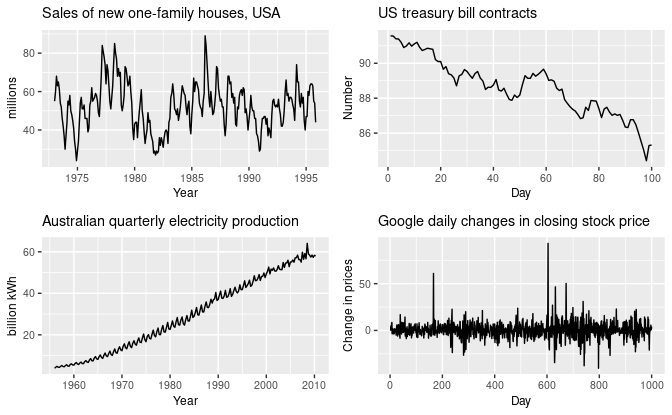
\includegraphics[width=\linewidth]{img/sota_ts_components.png}
	\caption{Four time series examples. Top left: seasonality and cycle; top right: trend only; bottom left: trend and seasonality; bottom right: random fluctuations}
	\end{figure}
	
	Trend and cycles are usually combined into a single trend-cycle component, often referred as trend for simplicity.
	Therefore, we can think of a time series as a combination of a trend-cycle component, a seasonal component, and a remainder component (containing anything else in the time series).
	By assuming additive decomposition we can write:\\\\
	\centerline{$y_t = S_t + T_t + R_t$}\\\\
	where $y_t$ is the data, $S_t$ the seasonal component, $T_t$ the trend component, and $R_t$ the remainder component, all at period $t$. When considering multiplicative decomposition, which occurs when the variation of the trend or of the seasonal component is proportional to the time series level, we can write: \\\\
	\centerline{$y_t = S_t * T_t * R_t$}\\
	To obtain such decomposition, STL \cite{STL} (Seasonal and Trend decomposition using Loess) can be applied, leading to the separation of trend, seasonality, and remainder as shown in figure \ref{fig:stl}.
	\begin{figure}[H]
		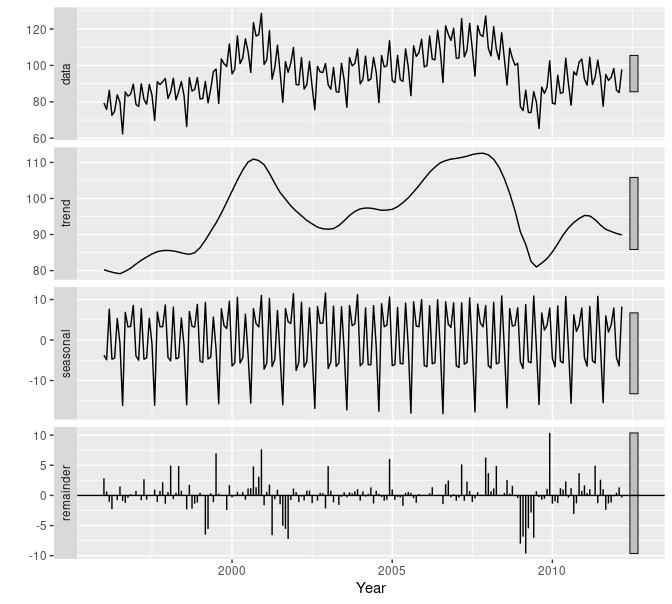
\includegraphics[width=\linewidth]{img/sota_ts_additive_decomposition.png}
		\caption{Additive decomposition of a time series using STL decomposition}
		\label{fig:stl}
	\end{figure}
	
	Given this background, let $Z=\{ z_{i, 1:T_i} \}_{i=1}^{N}$ be a  set of $N$ univariate time series where $z_{i, 1:T_i} = (z_{i,1}, z_{i,2}, ..., z_{i,T_i})$ and $z_{i,t} \in \mathbb{R}$ is the value of the $i$-th time series at time $t$. The time series may not have equally spaced points and do not have to be aligned (i.e. $t=1$ can refer to different absolute time points for different time series). Furthermore, let $X=\{ x_{i, 1:T_i+\tau} \}_{i=1}^{N}$ be a set of associated, time-varying covariate vectors with $\pmb{x}_{i,t} \in \mathbb{R}^D$ being e.g. a holiday flag or other useful information that must be known before computing the forecast up to time $T_i + \tau$.\\
	The goal of forecasting \cite{ForecastingHyndmanAthanasopoulos} is to predict the probability distribution of future values $z_{i,T_{i}+1:T_i+\tau}$ given the past values $z_{i, 1:T_i}$, the covariates $\pmb{x}_{i, 1:T_i + \tau}$, and the model parameters $\Phi$:
	\begin{equation} \label{eq:forecasting}
		p(z_{i,T_{i}+1:T_i+\tau} | z_{i, 1:T_i}, \pmb{x}_{i, 1:T_i + \tau}, \Phi)
	\end{equation}
	which can be reduced to point forecast by simply considering the conditional mean. The choice between probabilistic and point forecast depends on the application: probabilistic forecast can be used for applications like anomaly detection or when the forecasting task has an asymmetric cost for over and under-predicting. \\
	Equation \ref{eq:forecasting} is a supervised learning problem where the model structure is usually fixed upfront and we want to learn the model parameters $\Phi$ using an optimization method such as maximum likelihood estimation.
	
	Univariate models learn the model parameters $\Phi$ for each individual time series, while multivariate models are capable of learning a single global model for multiple time series by sharing the parameters.\\
	As noted by the latest M5 competition \cite{M5Competition}, nowadays time series models are typically sufficient for identifying and capturing their historical data pattern, i.e. level, trend, and seasonality. However, relying solely on historical data fails to effectively account for the effects of holidays and special events. Moreover, such factors can affect historical data, leading to distorted time series and consequently models. In such settings, the information from exogenous/explanatory variables, i.e.  $\pmb{x}_{i, 1:T_{i+\tau}}$, becomes of critical importance to improve accuracy; in fact, recent models such as the ones discussed later \cite{FacebookProphet, DeepAR, DeepState} allow the inclusion of these kind of variables.
	
	Time series models can be categorized as generative and discriminative \cite{DiscriminativeGenerativeModels}:\\
	\begin{center} \label{table:generativediscriminative}
		\begin{tabular}{ | c | c |}
			\hline
			Category & Modeling \\
			\hline
			Generative & $p(z_{i,1:T_i+\tau} | \pmb{x}_{i, 1:T_i + \tau}, \Phi)$ \\
			\hline
			Discriminative & $p(z_{i,T_{i}+1:T_i+\tau} | z_{i, 1:T_i}, \pmb{x}_{i, 1:T_i + \tau}, \Phi)$ \\
			\hline
		\end{tabular}
	\end{center}
	Generative models assume that time series are generated from an unknown stochastic process with some parametric structure of parameters $\Phi$ given the covariates $X$, while discriminative models model the conditional distribution for a fixed horizon $\tau$. The latter type of models is usually more flexible since they make less structural assumptions \cite{GluonTS}.
	
	
	\subsubsection{Exponential Smoothing} \label{sssec:exponential_smoothing}
	Exponential smoothing \cite{ExponentialSmoothingHoltCharles} is one of the oldest forecasting techniques that belongs to the generative models class (see \ref{table:generativediscriminative}). It is a lightweight means of smoothing random fluctuations using declining weights on older data, it's easy to compute and requires minimum data.
	The simplest form of exponential smoothing assumes that all past observations have equal importance:\\\\
	\centerline{$\hat{y}_{T+1|T} = \frac{1}{T} \sum_{t=1}^{T}y_t$}\\\\
	Where $\hat{y}_{T+1|T}$ is the forecasted value at time $T+1$ knowing past values up to time $T$. By introducing decaying weights, the formula becomes:\\\\
		\centerline{$\hat{y}_{T+1|T} = A(y_T + B y_{t-1} + B^2 y_{t-2} + B^3 y_{t-3} + ...)$ }\\\\
	where $A \in [0,1]$ and $B=1-A$, $A$ can attenuate the effect of old observations. The formula can be recursively applied to obtain observation at $T+k$, $k>1$. \\
	Exponential smoothing has been extended to take into consideration linear trend and seasonality \cite{ExponentialSmoothingHoltCharles} using the same equation above by approximating the trend at time $t$ as $y_t -y_{t-1}$ and knowing the seasonality period.\\
	Due to its nature, forecasts produced with this method will lag behind the actual trend.
	
	
	Exponential smoothing has been extended to take into consideration linear trend and seasonality \cite{ExponentialSmoothingHoltCharles}, both either additive or multiplicative. Trend can be damped, i.e. it can flatten over time converging to a maximum value, which can be useful for time series that exhibit a maximum "capacity" like the number of users limited by the Earth's population. 
	Seasonality period(s) must be given as input to the model.
	
	A state space approach, called Innovation State Space Model (ISSM) \cite{ExponentialSmoothingStateSpace}, has been proposed to add a statistical model that describes the data generation process, therefore providing prediction intervals. ISSM maintains a latent state vector $l_t$ with recent information about level, trend and seasonality. The state $l_t$ evolves over time adding a small innovation at each time step (i.e. the Gaussian noise):\\\\
	\centerline{$l_t = F_t l_{t-1} + g_t \epsilon_t$, $\epsilon_t \sim \mathcal{N}$}\\\\
	where $g_t$ controls innovation strength, making the observations a linear combination of the components of the current state. The parameters of ISSM are typically learned using the maximum likelihood principle.
	
	
	
	\subsubsection{ARMA models} \label{sssec:arma}
	
	ARMA models are auto-regressive models with a moving-average component, they provide a complementary approach to Exponential Smoothing and they belong to the generative models class (see \ref{table:generativediscriminative}). \\
	The Auto Regressive of order $p$ ($\text{AR}(p)$) component predicts the next value using a linear combination of $p$ previous known values, while the Moving Average of order $q$ ($\text{MA}(q)$) component takes into consideration the average and the last $q$ differences between the predicted and the actual value.  When combined, they form an ARMA$(p, q)$ model:\\\\
	\centerline{$\hat{y}_{t} = \text{ARMA}(p, q) = \text{AR}(p) + \text{MA}(q)  = \sum_{i=1}^{p}\phi_i y_{t-i} + \mu + \epsilon_t + \sum_{i=1}^{q}\theta_i \epsilon_{t-i} $}\\\\
	Unfortunately, ARMA requires the time series to be stationary, i.e. without trends and seasonality. To make a time series stationary and apply ARMA models, Box and Jenkins \cite{BoxJenkins} proposed an approach by: (1) providing guidelines for making the time series stationary, (2)  suggesting the use of autocorrelations and partial autocorrelation for determining appropriate values for $p$ and $q$, (3) providing a set of computer programs to identify appropriate values for $p$ and $q$, and (4) estimating the parameters involved. The approach is known as the Box-Jenkins methodology to ARIMA models, where the letter 'I' means 'Integrated', reflecting the need for differencing the time series to make it stationary. Furthermore, ARIMA can deal with seasonality by applying seasonal differencing, but requires the seasonality period to be known beforehand. This extension is called SARIMA.
	
	The more general SARIMA$(p, d, q, P, D, Q, m)$ model is defined by 7 parameters:
	\begin{itemize}
		\item $p$: trend auto-regression order
		\item $d$: trend difference order
		\item $q$: trend moving average order
		\item $P$: seasonal auto-regressive order
		\item $D$: seasonal difference order
		\item $Q$: seasonal moving average order
		\item $m$: seasonal period steps
	\end{itemize}

	Besides the availability of the well defined 3-steps Box-Jenkins framework, a lot of human work was still required to find the right values for these parameters. To tackle this issue many approaches have been developed, some of them being made available only by commercial software.  A well known automated solution has been implemented by \cite{AutoForecasting}, where they make use of unit root tests to find the differencing orders and the Akaike's information criterion (AIC) to select the best combination of $p$, $q$, $P$, and $Q$. AIC introduces a model complexity penalty to avoid overfitting data.\\
	Nevertheless, the number of steps of the seasonal period must still be given by the human, although it's often a well known seasonality (e.g. daily, weekly, yearly). Finally, SARIMA can only model one seasonality at a time.
		
	The vector ARIMA (VARIMA) model has been proposed as a multivariate generalization of the univariate ARIMA model, but in general Vector Auto-Regressive (VAR) models tend to suffer from overfitting, providing poor out-of-sample forecasts \cite{25YearsForecasting}.
	
	\subsubsection{ Prophet }
	Prophet \cite{FacebookProphet} is a solution developed by Facebook that provides an "analyst-in-the-loop" approach and a flexible model that fit a wide range of business time series. The model provided by Prophet aims at being configurable even by non-domain experts, simplifying the process of adding domain knowledge about the data generation process and heavily reducing the time required to obtain high quality forecasts.\\
	Figure \ref{fig:analyst_in_the_loop} shows a modeling step with straightforward human interpretation of the parameters followed by an evaluation process that provides a feedback. Finally, Prophet aims at being able to handle time series with trend changes, multiple seasonality, and holidays effects.
	\begin{figure}[H]
		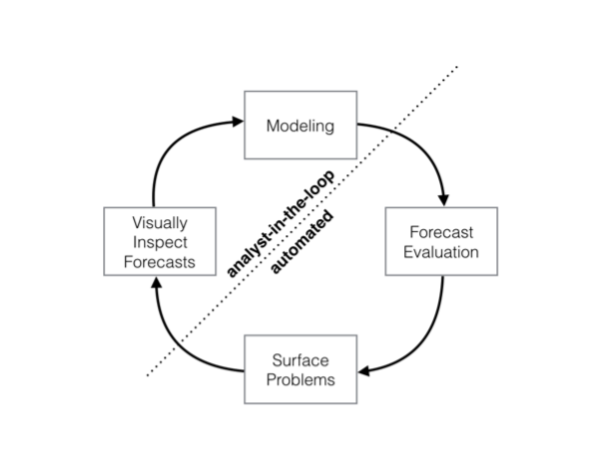
\includegraphics[width=\linewidth]{img/sota_ts_fb_prophet.png}
		\caption{Prophet analyst-in-the-loop approach}
		\label{fig:analyst_in_the_loop}
	\end{figure}
	Prophet model is a generalized additive model (GAM) \cite{GAM} that decomposes trend, seasonality, and holiday combining them in the following equation:\\\\
	\centerline{$y(t) = g(t) + s(t) + h(t) + \epsilon_t$}\\\\
	where $g(t)$ is the trend function which models non-periodic changes, $s(t)$ is the seasonality function that models periodic changes like daily and weekly seasonality, and $h(t)$ represents the effect of holidays which occur on potentially irregular schedules. Finally, the error term $\epsilon_t$ represents anything not accommodated by the model, which is assumed to be normally distributed. \\
	The advantage of using GAM formulation is that the model is capable of including new components as necessary, fitting very quickly by using, for example, L-BFGS. Therefore, the forecasting problem becomes a curve-fitting problem that is flexible, allows non-regularly spaced measurements, and is easily interpretable.\\
	The trend model $g(t)$ can be a saturating growth model capable of dealing with population growth (e.g. the number of subscriptions limited by the population of a country) or a piece-wise linear model.
	The latter has the following form:\\\\
	\centerline{$g(t) = (k+\pmb{a}(t)^T\pmb{\delta})t + (m + \pmb{a}(t)^T\gamma)$}\\\\
	where $k$ is the growth rate, $\pmb{\delta}$ has the rate adjustments, $m$ is the offset parameter, and $\gamma_j$ is set to $-s_j\delta_j$ to make the function continuous.\\
	Therefore, $\pmb{\delta} \in \!R^S$ defines $S$ trend change points occurring at time $s_j$, with $\delta_j$ being the rate adjustment. The rate at time $t$ is $k+\sum_{j:t>s_j}\delta_j$, which is more cleanly defined by a vector $\pmb{a}(t) \in \{0,1\}^S$ such that:\\\\
	\centerline{
		$
		a_j(t) =
		\begin{cases}
			1 & \text{if $t \geq s_j$}\\
			0 & \text{otherwise}
		\end{cases}       
		$
	}\\\\
	that makes the rate at time $t$ be $k + \pmb{a}(t)^T\pmb{\delta}$\\
	The change points $s_j$  can be specified by the analyst or they can be automatically selected by putting a sparse prior on $\pmb{\delta}$, e.g. a Laplace prior.\\
	The seasonality function $s(t)$ is modeled using Fourier series, meaning that a seasonality with period $P$ can be approximated by:\\\\
	\centerline{$s(t) = \sum_{n=1}^{N} (a_n \cos{(\frac{2\pi nt}{P})} + b_n \sin{(\frac{2\pi nt}{P})}) $}\\\\
	which can be automatically estimated finding $2N$ parameters, i.e. $\pmb{\beta} =  [a_1, b_1, ..., a_N, b_N]$. By choosing $N$, the series can be truncated at different depths allowing to fit seasonal patterns that change more or less quickly, possibly leading to overfitting. Finally, the initialization $\pmb{\beta} \sim \text{Normal}(0, \sigma^2)$ allows to impose a prior on the seasonality by choosing $\sigma$. \\
	The holiday model $h(t)$ that models somewhat predictable shocks is required because these kind of events is not well modeled by a smoothed Fourier series (events like Easter don't have a specific date). An analyst can provide a list of dates of interest $D_j$ for each holiday $j$, so the holiday model becomes:\\\\
	\centerline{$h(t) = Z(t) \pmb{\kappa}$}\\\\
	with $Z(t) = [ \mathbf{1} (t \in D_1), ..., \mathbf{1} (t \in D_L)] $ and $\pmb{\kappa}$ initialized as $\pmb{\kappa} \sim \text{Normal}(0, v^2)$, like it was done with seasonality.\\
	The Prophet solution is capable of achieving lower prediction errors when compared to traditional methods like Exponential Smoothing and ARIMA, with very quick fitting time.
	
	\subsubsection{ML models}
	The forecasting field has seen past practitioners proposing novel neural networks (NN) architectures that could not be considered competitive against simpler univariate statistical models. However, we are now living in the Big Data era: companies have gathered huge amounts of data over the years containing important information about their business patterns unlocking the possibility of learning effective multivariate models. Big data in the context of time series doesn't necessarily mean having single time series with with a lot of historical data, but it rather means that there are many related time series from the same domain \cite{RNNForecasting}. In such context, models capable of learning from multiple time series have emerged \cite{M5Competition} and proved to be able to outperform traditional ones.
	
	All recent successful models are based on Recurrent Neural Networks (RNN) \cite{RNN, RNNForecasting}, which demonstrated state-of-the-art performance in various applications handling sequential data like text, audio, and video where some kind of state must be kept while processing data. RNNs are a combination of recurrent units, e.g. Long Short-Term Memory (LSTM) and Gated Recurrent Unit (GRU) (see figure \ref{fig:lstmgru}). 
	\begin{figure}[H]
		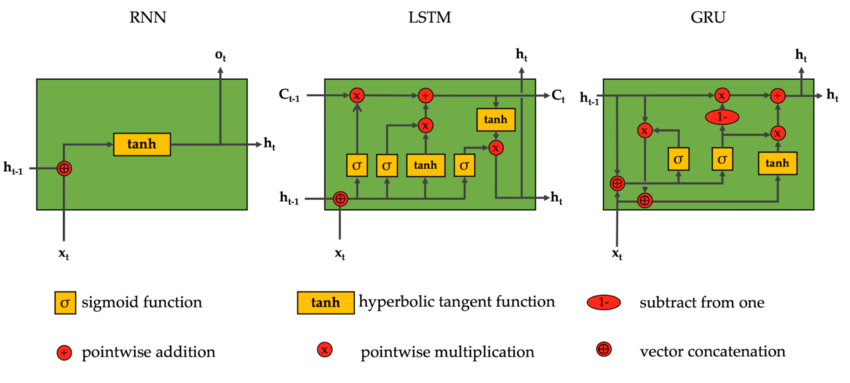
\includegraphics[width=\linewidth]{img/rnns.png}
		\caption{Architecture of an Elman recurrent unit, LSTM, and GRU. The output at step $t-1$ influences the output at step $t$.}
		\label{fig:lstmgru}
	\end{figure}
	By using recurrent edges connecting adjacent time steps (i.e. feedback loops), RNNs introduce the notion of time to the model: at time step $t$ the network receives the current input $\pmb{x}^{(t)}$ plus the previous network state $\pmb{h}^{(t-1)}$. \\
	RNNs are capable of producing both an output and a context (often called hidden state), where the context should act as memory of what has been seen by the network so far. Considering the simplest Elman recurrent unit, the hidden state $\pmb{h}^{(t)} \in \mathbb{R}^d$ ($d$ is the cell dimension) is computed as:\\
	\centerline{
	$
	\pmb{h}^{(t)} = \sigma(W_i \cdot \pmb{h}^{(t-1)} + V_i \cdot \pmb{x}^{(t)} + \pmb{b})
	$
	}\\
	where $\sigma$ is the activation function (e.g. \textit{tanh}), $\pmb{x}^{(t)} \in \mathbb{R}^m$ is the input, $W_i, V_i \in \mathbb{R}^{d \times d}$ are the weight matrices, and $\pmb{b} \in \mathbb{R}^{d}$ is the bias vector.
	
	Recurrent units (LSTM, GRU) can constitute RNNs in various types of architectures. A popular architecture is the forecasting field is Sequence to Sequence (S2S) \cite{seq2seq} which is commonly made of two RNNs: an encoder followed by a decoder. The encoder is used to extract features from known time series data (e.g. last day data points), and the decoder uses the information captured by the encoder to produce forecasts. Examples of models that make use of S2S are DeepAR \cite{DeepAR} and Multi-Horizon Quantile Recurrent Forecaster \cite{MQCNN}, explained later.
	
	By defining an encoder and a decoder, a model is allowed to see a limited amount of past values and can predict a fixed horizon, which means that any context and prediction length change requires re-training. Furthermore, many forecasting problems have long periodicity (e.g. 365 days) and may suffer memory loss during forward propagation. To overcome the long-dependency issue \cite{NARX} proposed a recurrent unit which computes a hidden state $h_t$ not only based on previous state $h_{t-1}$ but also a specific set of other past states (e.g. $(h_{t-2}), ..., h_{t-D}$) facilitating the ability of memorizing long dependencies. This technique is called skip-connection. However, the naive alternative adopted by \cite{DeepAR, MQCNN} obtains the same effect by feeding past time series values $(y_{t-1}, ..., y_{t-D})$ as feature inputs.
	
	More generally, the idea of feeding both time-dependent and time-independent features as input, along with the time series data points, has proven to be successful: when dealing with huge datasets, assigning time-independent (or static) features such as the category of the time series (e.g. "clothing" in the context of shopping) allow the model to learn both global and category-specific patterns, while time-dependent (or dynamic) features like day of week, holidays, and relevant events allow the model to learn and distinguish seasonality patterns from one-shot events, reducing the risk of overfitting. However, such dynamic features must be known beforehand when computing forecasts.
	
	The usage of such combination of features facilitates the learning of a global model exploiting information from many time series simultaneously. For NNs this means that weights are learned globally, but the state is maintained for each time series. Furthermore, the global model can be used to forecast time series that have never been seen during training and lack of data, as the model can still exploit patterns learned from the training set.
	
	
	
	
	% TODO introduction about RNNs - characteristics e.g. of LSTM - see https://arxiv.org/pdf/1705.04378.pdf , background of https://arxiv.org/pdf/1703.04691.pdf
	 
	% TODO add difference with traditional models like ARIMA: they make explicit assumptions -> no flexibility, they need a priori knowledge of the system
	
	% TODO add covariates details from https://arxiv.org/pdf/1711.11053.pdf
	
	\subsubsection{ DeepAR }
	DeepAR is a discriminative model 
	
	\subsection{ DeepState }
	DeepState is a generative model that combines state space models \cite{ExponentialSmoothingStateSpace} (see \ref{sssec:exponential_smoothing} for further details) with deep learning. The goal is to use a latent state $\pmb{l}_t \in \mathbb{R}^D$ to encode time series components such as level, trend, and seasonality patterns, and parametrize the linear state space model (SSM) by using a recurrent neural network (RNN) whose weights are learned jointly from multiple time series and covariates. 
	
	\subsection{ Workload forecasting }
	% ADD stuff about short term load forecasting (STLF) see https://arxiv.org/pdf/1705.04378.pdf
		When considering a time series, it may be useful to correlate it to another time series: for example, electricity demand could be affected by temperature (higher temperatures imply more air conditioner usages).  Correlation coefficients can be used to measure the relationship between two variables $x$ and $y$ is given by:
	
	$r = \frac{\sum{(x_t - \bar x)(y_t - \bar y)}}{\sqrt{\sum{(x_t - \bar x)^2}}\sqrt{\sum{(y_t - \bar y)^2}}}$
	
	\section{ Solution / Approach / Design }
	
	\section{ Experimental setup }
	
	\section{ Results }
	
	\section{ Conclusions }
	
	\section{ Future work }
		
	
	\newpage
	\bibliography{bibliography.bib} 
	\bibliographystyle{ieeetr}
	
	\end{document}
